\documentclass[conference]{IEEEtran}
\IEEEoverridecommandlockouts

\usepackage[utf8]{inputenc}
\usepackage[T1]{fontenc}
\usepackage[spanish,es-tabla,es-nodecimaldot,es-noquoting,es-noindentfirst]{babel}
\usepackage{cite}
\usepackage{amsmath,amssymb}
\usepackage{graphicx}
\usepackage{booktabs}
\usepackage{multirow}
\usepackage{xcolor}
\usepackage{url}
\usepackage{tikz}
\usepackage{balance}
\usetikzlibrary{positioning,arrows.meta,fit,calc,babel}

\definecolor{rUno}{HTML}{EB6834}
\definecolor{rDos}{HTML}{1BAF7A}
\definecolor{rTres}{HTML}{2A78D6}
\definecolor{rCuatro}{HTML}{E87BA4}
\renewcommand{\IEEEkeywordsname}{Palabras clave}

\begin{document}

\title{Rectificar o ajustar: detección de objetos en cámaras \textit{fisheye} de vehículos}

\author{\IEEEauthorblockN{Franco Marcelo Morero, Nicolás Granato, Marcos Levi Riveros Koloszwa y Tadeo Riveros Koloszwa}
\IEEEauthorblockA{Carrera de Especialización en Inteligencia Artificial (CEIA), Facultad de Ingeniería, Universidad de Buenos Aires\\
Visión por Computadora II, grupo 1}}

\maketitle

\begin{abstract}
Las cámaras de visión envolvente de los vehículos usan lentes \textit{fisheye} de casi 190°, que deforman los objetos hacia los bordes de la imagen. Un detector preentrenado en imágenes comunes pierde allí la mayor parte de su desempeño. Se compararon dos formas de adaptarlo: rectificar la imagen con una proyección cilíndrica y hacer \textit{fine-tuning} sobre las imágenes \textit{fisheye}. Las cuatro combinaciones de las dos estrategias usan el mismo YOLO11m, los mismos datos de WoodScape y la misma métrica, el mAP por anillos del ángulo de incidencia, sobre 1000 imágenes de prueba. Sin adaptar, el detector pierde el 69\,\% de su mAP@50 entre el centro y la periferia. El \textit{fine-tuning} sube la periferia de 0,170 a 0,603, reduce esa caída al 14\,\% y no agrega latencia. Rectificar mejora al detector preentrenado, pero empeora al ajustado, porque las cajas que vuelven a la imagen original quedan más grandes que los objetos. Un aumento de datos con distorsión radial no cambia el resultado con las mismas lentes, pero reduce a la mitad la pérdida con lentes distintas.
\end{abstract}

\begin{IEEEkeywords}
cámaras \textit{fisheye}, detección de objetos, \textit{fine-tuning}, proyección cilíndrica, WoodScape, YOLO11
\end{IEEEkeywords}

% =====================================================================
\section{Introducción}

\begin{figure*}[t]
\centering
\resizebox{\textwidth}{!}{%
\begin{tikzpicture}[
  font=\footnotesize, >={Stealth[length=4pt]}, x=1mm, y=1mm,
  caja/.style={draw=black!55, rounded corners=2pt, minimum height=6mm, inner xsep=0pt, inner ysep=2pt, align=center, fill=white},
  ent/.style={caja, text width=20mm},
  proc/.style={caja, text width=28mm},
  det/.style={caja, text width=47mm},
  sal/.style={caja, text width=40mm},
  eti/.style={font=\footnotesize\bfseries, minimum width=7mm, minimum height=6mm, text=white, rounded corners=2pt},
  flecha/.style={->, draw=black!60}]
  % columnas fijas: todas las cajas de una columna tienen el mismo ancho y centro
  \foreach \i/\c/\n in {1/rUno/R1, 2/rDos/R2, 3/rTres/R3, 4/rCuatro/R4} {
    \node[eti, fill=\c] (e\i) at (0, -10*\i) {\n};
    \node[ent] (f\i) at (19, -10*\i) {imagen \textit{fisheye}};
  }
  \node[proc] (p2) at (49, -20) {proyección cilíndrica};
  \node[proc] (p4) at (49, -40) {proyección cilíndrica};
  \node[det] (d1) at (93, -10) {YOLO11m preentrenado en COCO};
  \node[det] (d2) at (93, -20) {YOLO11m preentrenado en COCO};
  \node[det, fill=rTres!10] (d3) at (93, -30) {YOLO11m ajustado en \textit{fisheye}};
  \node[det, fill=rCuatro!12] (d4) at (93, -40) {YOLO11m ajustado en cilíndrica};
  \node[sal] (s1) at (142, -10) {cajas en la \textit{fisheye}};
  \node[sal] (s2) at (142, -20) {cajas de vuelta a la \textit{fisheye}};
  \node[sal] (s3) at (142, -30) {cajas en la \textit{fisheye}};
  \node[sal] (s4) at (142, -40) {cajas de vuelta a la \textit{fisheye}};
  \node[caja, minimum height=36mm, text width=33mm] (ev) at (186, -25)
    {Evaluación común\\[1pt] mAP@50, mAP@50-95\\ por anillo de $\theta$\\ (esquema de COCO)\\[1pt] latencia en la misma máquina};
  \draw[flecha] (f1) -- (d1); \draw[flecha] (f3) -- (d3);
  \draw[flecha] (f2) -- (p2); \draw[flecha] (p2) -- (d2);
  \draw[flecha] (f4) -- (p4); \draw[flecha] (p4) -- (d4);
  \foreach \i in {1,2,3,4} { \draw[flecha] (d\i) -- (s\i); \draw[flecha] (s\i.east) -- (ev.west |- s\i); }
\end{tikzpicture}}
\caption{Diseño factorial $2\times2$. R1 aplica el detector preentrenado sobre la imagen original. R2 aplica el mismo detector sobre la proyección cilíndrica y devuelve las cajas a la imagen \textit{fisheye}. R3 hace \textit{fine-tuning} sobre la imagen \textit{fisheye} y R4, sobre la proyección cilíndrica. Las cuatro ramas se evalúan con la misma métrica sobre la imagen original.}
\label{fig:ramas}
\end{figure*}


Los sistemas de visión envolvente (\textit{surround view}) combinan cuatro cámaras \textit{fisheye}, una frontal, una trasera y una en cada espejo, que cubren 360° alrededor del vehículo. Con ellas funcionan el estacionamiento automático, la asistencia en atascos y la conducción urbana~\cite{kumar2023survey}. La lente sigue un modelo de proyección polinomial en $\theta$, como el de Kannala y Brandt~\cite{kannala2006}. En WoodScape es de cuarto orden, $\rho(\theta)=k_1\theta+k_2\theta^2+k_3\theta^3+k_4\theta^4$~\cite{yogamani2019woodscape}, y en él la deformación de un objeto depende del ángulo de incidencia $\theta$ respecto del eje óptico. Un peatón a 20° y el mismo peatón a 85° tienen geometrías muy distintas en la imagen. Los detectores disponibles se preentrenan en imágenes de perspectiva, como las de COCO (\textit{Common Objects in Context})~\cite{lin2014coco}, y por eso resuelven peor la periferia, que es la zona más importante para la seguridad.

La industria automotriz ya trabaja sobre este problema. Valeo publicó WoodScape~\cite{yogamani2019woodscape}, el primer conjunto de datos público extenso de cámaras \textit{fisheye} automotrices. Sobre ese conjunto, su equipo desarrolló OmniDet (2021)~\cite{kumar2021omnidet}, una red de percepción multitarea para las cuatro cámaras que funciona en tiempo real en \textit{hardware} embebido automotriz (NVIDIA Jetson AGX con TensorRT). Fuera del vehículo, FishEye8K (2023)~\cite{gochoo2023fisheye8k} reúne 8000 imágenes de 18 cámaras \textit{fisheye} que monitorean el tránsito en calles e intersecciones de Hsinchu, Taiwán, para detectar autos, autobuses, camiones, bicicletas y motos, y peatones. En los dos casos el detector trabaja sobre la imagen deformada.

Las soluciones se agrupan en dos familias. La primera rectifica la imagen y usa el detector sin cambios. Plaut et al.~\cite{plaut2021cylindrical} mostraron que una proyección cilíndrica permite aplicar detectores entrenados solo con imágenes de perspectiva. La segunda adapta el modelo con datos \textit{fisheye}, y Rashed et al.~\cite{rashed2021generalized} señalaron además que la caja rectangular representa mal a los objetos deformados. Para un equipo que parte de un detector preentrenado, la pregunta práctica es cuál de las dos conviene y si vale la pena combinarlas. Los trabajos previos suelen evaluar una sola estrategia, con modelos, datos o métricas distintos, y eso impide compararlas.

El objetivo del trabajo es medir cuánto aporta rectificar, cuánto aporta el \textit{fine-tuning} y cómo interactúan, con el mismo detector, los mismos datos y la misma métrica, y con foco en la periferia y en la latencia. Las contribuciones son las siguientes:
\begin{itemize}
\item Un diseño factorial $2\times2$ que cruza rectificar o no con hacer \textit{fine-tuning} o no, para separar los dos efectos y estimar su interacción.
\item Una métrica que separa los objetos según su ángulo de incidencia $\theta$, es decir, según qué tan lejos del centro de la lente caen. Sigue el esquema de evaluación de COCO, está validada contra \texttt{pycocotools} y usa una partición controlada para que no haya imágenes casi iguales entre entrenamiento y prueba.
\item La evidencia de que rectificar resta una vez que el modelo se adapta, con una explicación cuantitativa: el límite de IoU (\textit{intersection over union}) que impone el regreso de las cajas a la imagen original.
\item Un aumento de datos con distorsión radial que no cambia el desempeño con las lentes del conjunto de datos, pero reduce a la mitad la pérdida con otras lentes.
\end{itemize}

% =====================================================================
\section{Metodología, diseño y desarrollo}

\subsection{Datos y partición}
Se usaron las 8234 imágenes públicas de WoodScape~\cite{yogamani2019woodscape}, de 1280$\times$966 píxeles, tomadas por las cámaras FV (\textit{front view}, frontal), MVL (\textit{mirror view left}, espejo izquierdo), MVR (\textit{mirror view right}, espejo derecho) y RV (\textit{rear view}, trasera), con 23 juegos de calibración intrínseca. Las 43 etiquetas de instancia se agrupan en tres clases: \texttt{vehicle} (\texttt{car}, \texttt{van}, \texttt{bus}, \texttt{truck}, \texttt{trailer} y \texttt{caravan}), \texttt{person} (\texttt{person} y \texttt{rider}) y \texttt{two\_wheeler} (\texttt{bicycle} y \texttt{motorcycle}). La caja de referencia es la envolvente del polígono de cada objeto. Se descartan las cajas menores a 300\,px$^2$ o con un lado menor a 8\,px.

WoodScape proviene de grabaciones continuas, así que un muestreo aleatorio podría repartir cuadros casi idénticos entre entrenamiento y prueba. Con \textit{hashes} perceptuales de 256 bits se verificó que la distancia mediana entre cada imagen de prueba y su vecina más cercana de entrenamiento es de 39 bits (15,2\,\%). El único par sospechoso quedó en cuarentena. La partición final, estratificada por cámara, tiene 6148 imágenes de entrenamiento, 1085 de validación y 1000 de prueba con 11\,910 objetos. Las imágenes se verifican por sha256 y nunca se recomprimen. La prueba no se usó para elegir \textit{checkpoint} ni hiperparámetros. Cada rama se evaluó sobre ella con sus pesos finales.

\subsection{Métrica estratificada por ángulo de incidencia}
Para cada caja se calcula el ángulo $\theta$ de su centro a partir de la calibración de su imagen. Se usa $\theta$ y no la distancia en píxeles al centro porque es lo que determina la deformación y vale igual para cámaras con calibraciones distintas. Las cajas se reparten en tres anillos: centro, medio y periferia. Los cortes, 68,3° y 80,7°, dejan 3970 objetos de la prueba en cada anillo y son los mismos para todas las ramas.

Cada anillo se evalúa como COCO evalúa cada rango de tamaño (\texttt{areaRng}), con $\theta$ en lugar del área. Los objetos de otros anillos se marcan \textit{ignore}, así que detectarlos no cuenta como acierto ni como falso positivo. Como control se usa también un esquema de filtrado, que descarta las cajas de referencia y las detecciones cuyo centro cae fuera del anillo.

Se reporta el mAP (\textit{mean average precision}) con umbral de IoU de 0,5 (mAP@50) y promediado entre 0,5 y 0,95 (mAP@50-95), con la configuración de COCO y un umbral de confianza de 0,01. El evaluador da los mismos valores que \texttt{pycocotools}. La latencia se mide por imagen en la misma máquina para las cuatro ramas, una Apple M4 Max con MPS (\textit{Metal Performance Shaders}), después de diez pasadas de calentamiento y sin contar la lectura del disco.

\subsection{Las cuatro ramas}
Las cuatro ramas (Fig.~\ref{fig:ramas}) usan YOLO11m~\cite{yolo11}, con 20,1\,M parámetros, 68,1\,GFLOPs y entrada de 640\,px. Se probaron ocho detectores preentrenados: YOLO11 en sus cinco tamaños, dos Faster R-CNN y una Mask R-CNN. YOLO11m fue el de mejor equilibrio entre precisión y latencia. Además, es un detector de una etapa, apto para una ECU (\textit{electronic control unit}). Todas las ramas se evalúan sobre la imagen \textit{fisheye} original, que es la que usa el vehículo.

\textit{R1, sin adaptar.} El detector se aplica directo sobre la imagen. Sus clases de COCO se traducen a las del trabajo: \texttt{car}, \texttt{bus} y \texttt{truck} pasan a \texttt{vehicle}, y \texttt{bicycle} y \texttt{motorcycle} pasan a \texttt{two\_wheeler}. La clase \texttt{person} se mantiene.

\textit{R2, rectificar.} La imagen pasa a una proyección cilíndrica de 190° horizontales~\cite{plaut2021cylindrical}, recortada a una banda de $\pm45^\circ$ alrededor del horizonte. Esa banda contiene el centro del 95,7\,\% de las cajas de prueba. No se usó la proyección de perspectiva porque lleva los píxeles cercanos a 90° a distancias infinitas~\cite{plaut2021cylindrical} y obliga a recortar la periferia, que es la zona en estudio.\footnote{E.~Plaut explica con ejemplos por qué la proyección de perspectiva no puede representar ángulos mayores a 90° y la cilíndrica sí, en su tutorial sobre visión por computadora con cámaras \textit{fisheye}: \url{https://plaut.github.io/fisheye_tutorial/}.} Para volver a la imagen \textit{fisheye}, cada caja detectada se recorre con 20 puntos por lado. Se descartan los puntos que caen fuera de la imagen y se toma la caja que encierra al resto.

\textit{R3, adaptar.} Se hace \textit{fine-tuning} de YOLO11m sobre las imágenes \textit{fisheye}, desde los pesos de COCO y con una cabeza nueva para las tres clases.

\textit{R4, ambas.} Se hace \textit{fine-tuning} sobre la proyección cilíndrica de R2. Para obtener las etiquetas se proyecta el polígono de cada objeto y se toma su caja en la imagen cilíndrica. Proyectar la caja de referencia la agrandaría en la periferia.

R3 y R4 se entrenan igual. Usan 30 épocas, un lote de 64 imágenes por acumulación de gradiente, AdamW con tasa de aprendizaje de 1,43$\times10^{-3}$ y los aumentos de datos por defecto de Ultralytics: mosaico, cambios de color, espejado, escala y traslación, sin mosaico en las 10 últimas épocas. En cada rama se guarda la época con mejor mAP@50-95 en validación. R3 se entrenó en una Apple M4 Max (3,4\,h), con 16 imágenes por paso. R4 se entrenó en una GTX 1660 de 6\,GB, con 2 imágenes por paso por falta de memoria y sin precisión mixta. También cambia la semilla.

\subsection{Extensión: aumento de datos con distorsión radial}
El modelo de R3 aprende las lentes de WoodScape. Para que funcione también con otras lentes, se entrenó una variante que deforma algunas imágenes al azar durante el entrenamiento. La deformación es una distorsión radial simétrica con un solo coeficiente $k$, del tipo que Brown describe con los coeficientes $K_1, K_2, \ldots$~\cite{brown1966}. Cada píxel a distancia $r$ del centro óptico toma el valor del punto a distancia
\begin{equation}
r_{\mathrm{src}}=r\,\frac{1+kr^2}{1+k}
\end{equation}
donde $r$ vale 1 en la esquina más lejana. Con $k>0$ la imagen se ve más \textit{fisheye} y con $k<0$, menos. En cada imagen se aplica con probabilidad 0,5 y con $k$ elegido al azar entre $-0{,}2$ y $0{,}3$, rango en el que la transformación no se pliega sobre sí misma. Las cajas se deforman igual que la imagen. Esta variante se entrenó con la misma configuración que R3.

% =====================================================================
\section{Resultados experimentales y análisis}

\subsection{Resultados por anillo}
La Tabla~\ref{tab:principal} y la Fig.~\ref{fig:anillos} muestran los resultados de las cuatro ramas. La caída es cuánto baja el mAP@50 del centro a la periferia, en porcentaje. Sin adaptar, R1 cae un 69\,\%. El problema no es de este detector en particular. YOLO26m~\cite{jocher2026yolo26}, una generación posterior, obtiene en la periferia casi lo mismo que YOLO11m, 0,171 contra 0,160 con el esquema de filtrado.

\begin{table}[t]
\centering
\caption{Resultados en las 1000 imágenes de prueba (mAP por anillo de $\theta$, esquema de COCO). La caída es la del mAP@50 del centro a la periferia. La latencia es la media por imagen en la misma máquina.}
\label{tab:principal}
\setlength{\tabcolsep}{3.2pt}
\begin{tabular}{@{}lccccccr@{}}
\toprule
 & \multicolumn{2}{c}{Global} & \multicolumn{3}{c}{mAP@50 por anillo} & & \\
\cmidrule(lr){2-3}\cmidrule(lr){4-6}
Rama & mAP@50 & 50-95 & centro & medio & perif. & caída & ms \\
\midrule
R1 sin adaptar      & 0,378 & 0,239 & 0,541 & 0,432 & 0,170 & 69\,\% & 25,0 \\
R2 cilíndrica       & 0,418 & 0,155 & 0,528 & 0,420 & 0,316 & 40\,\% & 26,6 \\
R3 \textit{fine-tuning} & \textbf{0,659} & \textbf{0,430} & \textbf{0,701} & \textbf{0,670} & \textbf{0,603} & \textbf{14\,\%} & \textbf{22,9} \\
R4 ambas            & 0,522 & 0,172 & 0,642 & 0,522 & 0,412 & 36\,\% & 28,6 \\
\bottomrule
\end{tabular}
\end{table}

\begin{figure}[t]
\centering
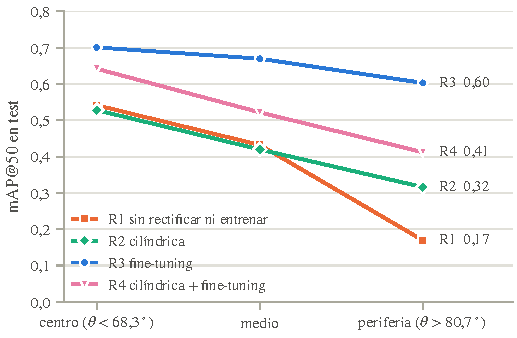
\includegraphics[width=\columnwidth]{figs/anillos.pdf}
\caption{mAP@50 por anillo de ángulo de incidencia en la prueba. R3, el \textit{fine-tuning} sin rectificar, es la única rama que se mantiene casi plana hacia la periferia.}
\label{fig:anillos}
\end{figure}

La caída se debe a la deformación y no al tamaño de los objetos. La Tabla~\ref{tab:tamano} separa los objetos por tamaño, con los rangos de área de COCO. En R1, los grandes bajan de 0,841 en el centro a 0,510 en la periferia ($-39$\,\%) y los pequeños, de 0,301 a 0,030 ($-90$\,\%). Es decir, la deformación afecta más a los objetos que ocupan pocos píxeles. El \textit{fine-tuning} mejora los tres tamaños. En la periferia, el mAP@50 de los objetos pequeños sube de 0,030 a 0,296.

\begin{table}[t]
\centering
\caption{mAP@50 por anillo y tamaño de objeto (rangos de área de COCO: pequeño $<32^2$, mediano $<96^2$ px). Entre paréntesis, la cantidad de objetos.}
\label{tab:tamano}
\setlength{\tabcolsep}{3.4pt}
\begin{tabular}{@{}lcccccc@{}}
\toprule
 & \multicolumn{3}{c}{Centro} & \multicolumn{3}{c}{Periferia} \\
\cmidrule(lr){2-4}\cmidrule(lr){5-7}
Rama & pequeño & mediano & grande & pequeño & mediano & grande \\
 & (1546) & (1790) & (634) & (1288) & (2147) & (535) \\
\midrule
R1 & 0,301 & 0,654 & 0,841 & 0,030 & 0,175 & 0,510 \\
R2 & 0,334 & 0,636 & 0,786 & 0,092 & 0,392 & 0,639 \\
R3 & \textbf{0,472} & \textbf{0,806} & \textbf{0,946} & \textbf{0,296} & \textbf{0,695} & \textbf{0,892} \\
R4 & 0,451 & 0,747 & 0,885 & 0,191 & 0,480 & 0,739 \\
\bottomrule
\end{tabular}
\end{table}

\subsection{Efectos del diseño factorial}
La Tabla~\ref{tab:efectos} compara pares de ramas que difieren en un solo factor. El \textit{fine-tuning} es el factor más importante: sin rectificar, suma 0,433 de mAP@50 en la periferia. Rectificar mejora al detector preentrenado en 0,147, pero al detector ajustado le resta 0,191. La interacción mide cuánto cambia el efecto de rectificar según haya o no \textit{fine-tuning}. Se calcula como $(\mathrm{R4}-\mathrm{R3})-(\mathrm{R2}-\mathrm{R1})$ y en la periferia vale $-0{,}337$. Se esperaba que rectificar aportara menos después del \textit{fine-tuning}, pero el resultado fue que empeora el desempeño. Esto se mantiene con otras formas de definir los anillos: la interacción es de $-0{,}339$ con el esquema de filtrado y de $-0{,}354$ con anillos por distancia al centro, cortados en un tercio y dos tercios de la media diagonal de la imagen.

\begin{table}[t]
\centering
\caption{Efectos del diseño $2\times2$ en la prueba (diferencias de mAP, anillos por $\theta$).}
\label{tab:efectos}
\setlength{\tabcolsep}{4pt}
\begin{tabular}{@{}lccc@{}}
\toprule
 & mAP@50 & mAP@50 & mAP@50-95 \\
Efecto & global & perif. & perif. \\
\midrule
Rectificar sin \textit{fine-tuning} (R2$-$R1) & $+0{,}041$ & $+0{,}147$ & $+0{,}010$ \\
Rectificar con \textit{fine-tuning} (R4$-$R3) & $-0{,}138$ & $-0{,}191$ & $-0{,}252$ \\
\textit{Fine-tuning} sin rectificar (R3$-$R1) & $+0{,}282$ & $+0{,}433$ & $+0{,}278$ \\
\textit{Fine-tuning} con rectificar (R4$-$R2) & $+0{,}104$ & $+0{,}096$ & $+0{,}016$ \\
\midrule
Interacción (R4$-$R3)$-$(R2$-$R1) & $\mathbf{-0{,}178}$ & $\mathbf{-0{,}337}$ & $\mathbf{-0{,}261}$ \\
\bottomrule
\end{tabular}
\end{table}

\begin{figure*}[t]
\centering
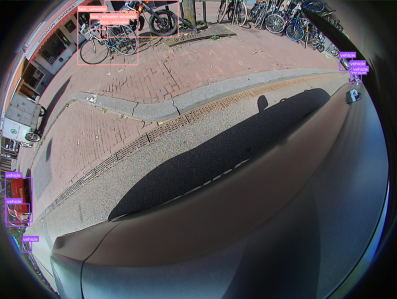
\includegraphics[width=0.32\textwidth]{figs/cual_gt.png}\hfill
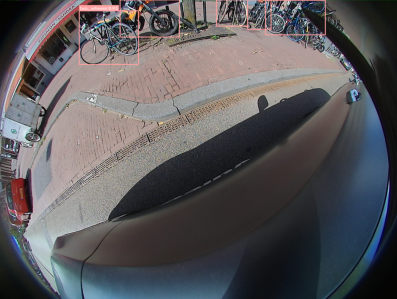
\includegraphics[width=0.32\textwidth]{figs/cual_r1.png}\hfill
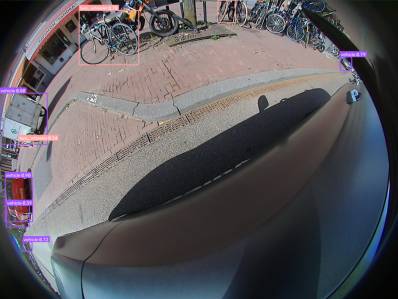
\includegraphics[width=0.32\textwidth]{figs/cual_r3.png}
\caption{Ejemplo ilustrativo de la cámara del espejo derecho (imagen 02794\_MVR, del conjunto de entrenamiento). Izquierda: referencia. Centro: R1 solo detecta las bicicletas del borde superior. Derecha: R3 detecta los autos estirados de la periferia izquierda y derecha (umbral de visualización 0,3).}
\label{fig:cualitativo}
\end{figure*}

\subsection{Por qué rectificar resta}
Las ramas rectificadas pierden sobre todo en mAP@50-95: R2 y R4 obtienen 0,155 y 0,172, contra 0,239 de R1 y 0,430 de R3. La causa es el paso de vuelta a la imagen original. Una caja recta en la proyección cilíndrica se vuelve curva en la imagen \textit{fisheye}, y la caja que la encierra queda más grande que el objeto.

Para medir cuánto se pierde así, se simuló una detección perfecta. El polígono de cada objeto se llevó a la proyección cilíndrica, se tomó su caja y se la devolvió a la imagen \textit{fisheye}. Aun así, la IoU mediana con la caja original fue de 0,81 en el centro y de 0,65 y 0,66 fuera de él, con anillos definidos por distancia al centro. Fuera del centro, entre el 6,9\,\% y el 11,6\,\% de los objetos no llega a IoU 0,5. Además, el 3,4\,\% de los objetos queda fuera de la banda cilíndrica y no se puede detectar.

El problema no está en el entrenamiento de R4. Sobre la proyección cilíndrica, R4 llega a 0,446 de mAP@50-95 en validación, casi lo mismo que R3 sobre la imagen \textit{fisheye} (0,431). Lo que pierde aparece al devolver las cajas, y ningún entrenamiento lo compensa. Con el detector preentrenado, en cambio, rectificar ayuda más de lo que cuesta, al menos con IoU 0,5.

\subsection{Cámaras, clases y ejemplo cualitativo}
Las cámaras laterales son las más afectadas (Tabla~\ref{tab:camaras}), porque miran hacia abajo y ven casi toda la calle en la periferia. R3 sube su mAP@50 de 0,26 a 0,60 en MVL y a 0,65 en MVR, más que lo que logra R1 con la cámara frontal. Por clase, en la periferia, \texttt{vehicle} pasa de 0,185 a 0,816, \texttt{person} de 0,207 a 0,507 y \texttt{two\_wheeler} de 0,117 a 0,486. La Fig.~\ref{fig:cualitativo} muestra un ejemplo con una imagen del conjunto de entrenamiento. El detector de COCO no encuentra los autos estirados en los bordes de una cámara lateral, y el modelo ajustado sí.

\begin{table}[t]
\centering
\caption{mAP@50 global por cámara en la prueba.}
\label{tab:camaras}
\setlength{\tabcolsep}{5pt}
\begin{tabular}{@{}lcccc@{}}
\toprule
Rama & FV (frontal) & MVL (izq.) & MVR (der.) & RV (trasera) \\
\midrule
R1 & 0,521 & 0,259 & 0,264 & 0,495 \\
R2 & 0,498 & 0,354 & 0,363 & 0,474 \\
R3 & \textbf{0,701} & \textbf{0,603} & \textbf{0,653} & \textbf{0,671} \\
R4 & 0,625 & 0,453 & 0,468 & 0,547 \\
\bottomrule
\end{tabular}
\end{table}


\subsection{Latencia}
Las cuatro ramas se midieron en la misma máquina y en la misma sesión (Tabla~\ref{tab:principal}). El detector tarda entre 23 y 25\,ms por imagen en todas, porque es el mismo modelo. Rectificar agrega unos 3\,ms, un 12\,\% más, para proyectar la imagen y devolver las cajas. El \textit{fine-tuning} no agrega tiempo, porque solo cambia los pesos. En otra sesión el mismo modelo tardó 17\,ms, pero las diferencias entre ramas se mantuvieron.

\subsection{Entrenamiento y aumento de datos con distorsión radial}
En R3, el mAP@50-95 de validación sube 0,123 entre las épocas 1 y 10, 0,062 entre la 10 y la 20, y 0,026 entre la 20 y la 30. Cada tramo aporta menos que el anterior. Tampoco hay sobreajuste, porque validación y prueba dan 0,652 y 0,659 de mAP@50. Entrenar más épocas sumaría centésimas, poco frente a los 0,43 que ya se ganaron en la periferia.

Con las lentes de WoodScape, el aumento de datos con distorsión radial no cambia el resultado. En la prueba da 0,656 de mAP@50 y 0,426 de mAP@50-95, contra 0,659 y 0,430 del modelo base. Su aporte aparece cuando cambia la lente (Fig.~\ref{fig:robustez}). Se deformaron 300 imágenes de validación con $k$ entre $-0{,}2$ y $+0{,}3$. El modelo base pierde hasta 0,062 de mAP@50-95 y el entrenado con el aumento, 0,027, menos de la mitad.

\begin{figure}[t]
\centering
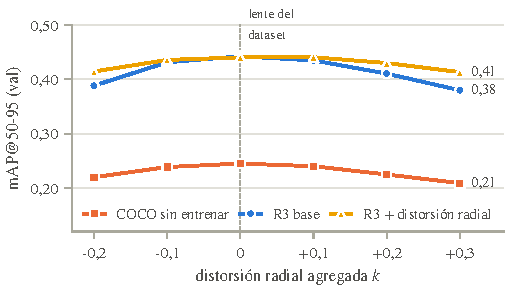
\includegraphics[width=\columnwidth]{figs/robustez.pdf}
\caption{Robustez a una distorsión radial agregada en validación (300 imágenes). En $k=0$ las tres curvas corresponden a la lente del conjunto de datos. Hacia la derecha la lente es más \textit{fisheye} y hacia la izquierda, menos.}
\label{fig:robustez}
\end{figure}

% =====================================================================
\section{Conclusiones}

Se compararon cuatro formas de usar YOLO11m sobre las cámaras \textit{fisheye} de WoodScape, con los mismos datos y la misma métrica. De los resultados se extraen las siguientes conclusiones:

\begin{enumerate}
\item El problema es la deformación de la lente y no el detector elegido. YOLO11m pierde el 69\,\% de su mAP@50 del centro a la periferia, en objetos de todos los tamaños. Un detector más nuevo, YOLO26m, rinde casi igual en la periferia.
\item La mejor estrategia es hacer \textit{fine-tuning} sobre la imagen \textit{fisheye}. Sube la periferia de 0,170 a 0,603 y el mAP@50 global de 0,378 a 0,659, mejora las cuatro cámaras y no agrega latencia, porque es el mismo modelo con otros pesos.
\item Rectificar la imagen solo sirve si no se hace \textit{fine-tuning}. Mejora al detector preentrenado en la periferia, pero empeora al modelo ajustado. Se esperaba que aportara poco después del \textit{fine-tuning}, no que restara.
\item Rectificar resta porque las cajas vuelven deformadas a la imagen original. Aun con una detección perfecta, la caja devuelta coincide poco con el objeto fuera del centro, y algunos objetos quedan fuera de la proyección. Cualquier método que rectifique, detecte y devuelva cajas tiene este límite.
\item Deformar las imágenes al entrenar no mejora el resultado con las lentes de WoodScape. Sí hace al modelo más robusto: con otras lentes pierde la mitad que sin ese aumento de datos. Esto sirve si los vehículos usan cámaras distintas.
\item Hay que evaluar por anillos de ángulo y sobre la imagen original. El mAP global esconde lo que pasa en la periferia, y medir cada rama en su propia imagen habría escondido el costo de rectificar. Las conclusiones no cambian con otras formas de definir los anillos.
\end{enumerate}

\textit{Trabajo futuro.} El estudio se puede extender en tres direcciones. La primera es repetir el diseño con otros detectores, de dos etapas o basados en \textit{transformers}. La segunda es rectificar de otra forma, con varias vistas de perspectiva o una proyección esférica. La tercera es usar cajas rotadas, elipses o polígonos, que siguen la forma deformada del objeto~\cite{rashed2021generalized}. Así, las ramas rectificadas podrían perder menos al volver a la imagen original.

% =====================================================================
\balance
\begin{thebibliography}{10}

\bibitem{yogamani2019woodscape}
S.~Yogamani, C.~Hughes, J.~Horgan, G.~Sistu, P.~Varley, D.~O'Dea, M.~U\v{r}i\v{c}\'a\v{r}, S.~Milz, M.~Simon, K.~Amende, C.~Witt, H.~Rashed, S.~Chennupati, S.~Nayak, S.~Mansoor, X.~Perrotton y P.~Pérez, ``WoodScape: A multi-task, multi-camera fisheye dataset for autonomous driving,'' en \emph{Proc. IEEE/CVF Int. Conf. Comput. Vis. (ICCV)}, 2019, pp.~9307--9317, doi: 10.1109/ICCV.2019.00940.

\bibitem{kumar2023survey}
V.~R. Kumar, C.~Eising, C.~Witt y S.~K. Yogamani, ``Surround-view fisheye camera perception for automated driving: Overview, survey \& challenges,'' \emph{IEEE Trans. Intell. Transp. Syst.}, vol.~24, no.~4, pp.~3638--3659, 2023, doi: 10.1109/TITS.2023.3235057.

\bibitem{kumar2021omnidet}
V.~R. Kumar, S.~K. Yogamani, H.~Rashed, G.~Sistu, C.~Witt, I.~Leang, S.~Milz y P.~Mäder, ``OmniDet: Surround view cameras based multi-task visual perception network for autonomous driving,'' \emph{IEEE Robot. Autom. Lett.}, vol.~6, no.~2, pp.~2830--2837, 2021, doi: 10.1109/LRA.2021.3062324.

\bibitem{rashed2021generalized}
H.~Rashed, E.~Mohamed, G.~Sistu, V.~R. Kumar, C.~Eising, A.~El-Sallab y S.~Yogamani, ``Generalized object detection on fisheye cameras for autonomous driving: Dataset, representations and baseline,'' en \emph{Proc. IEEE/CVF Winter Conf. Appl. Comput. Vis. (WACV)}, 2021, pp.~2271--2279, doi: 10.1109/WACV48630.2021.00232.

\bibitem{plaut2021cylindrical}
E.~Plaut, E.~Ben-Yaacov y B.~El~Shlomo, ``3D object detection from a single fisheye image without a single fisheye training image,'' en \emph{Proc. IEEE/CVF Conf. Comput. Vis. Pattern Recognit. Workshops (CVPRW)}, 2021, pp.~3654--3662, doi: 10.1109/CVPRW53098.2021.00405.

\bibitem{gochoo2023fisheye8k}
M.~Gochoo, M.-E. Otgonbold, E.~Ganbold, J.-W. Hsieh, M.-C. Chang, P.-Y. Chen, B.~Dorj, H.~Al~Jassmi, G.~Batnasan, F.~Alnajjar, M.~Abduljabbar y F.-P. Lin, ``FishEye8K: A benchmark and dataset for fisheye camera object detection,'' en \emph{Proc. IEEE/CVF Conf. Comput. Vis. Pattern Recognit. Workshops (CVPRW)}, 2023, pp.~5305--5313, doi: 10.1109/CVPRW59228.2023.00559.

\bibitem{kannala2006}
J.~Kannala y S.~S. Brandt, ``A generic camera model and calibration method for conventional, wide-angle, and fish-eye lenses,'' \emph{IEEE Trans. Pattern Anal. Mach. Intell.}, vol.~28, no.~8, pp.~1335--1340, 2006, doi: 10.1109/TPAMI.2006.153.

\bibitem{lin2014coco}
T.-Y. Lin, M.~Maire, S.~Belongie, J.~Hays, P.~Perona, D.~Ramanan, P.~Dollár y C.~L. Zitnick, ``Microsoft COCO: Common objects in context,'' en \emph{Proc. Eur. Conf. Comput. Vis. (ECCV)}, 2014, pp.~740--755, doi: 10.1007/978-3-319-10602-1\_48.

\bibitem{yolo11}
G.~Jocher y J.~Qiu, ``Ultralytics YOLO11,'' versión 11.0.0, 2024. [En línea]. Disponible: \url{https://github.com/ultralytics/ultralytics}

\bibitem{brown1966}
D.~C. Brown, ``Decentering distortion of lenses,'' \emph{Photogramm. Eng.}, vol.~32, no.~3, pp.~444--462, 1966.

\bibitem{jocher2026yolo26}
G.~Jocher, J.~Qiu, M.~Liu, S.~Lyu, F.~C. Akyon y M.~E. Kalfaoglu, ``Ultralytics YOLO26: Unified real-time end-to-end vision models,'' arXiv:2606.03748, 2026, doi: 10.48550/arXiv.2606.03748.

\end{thebibliography}

\end{document}
